In~\cite{cruz-ppdp14} we described the structure and organization of the virtual
that allows LM programs to be run in parallel. In this section, we review the
the supporting runtime that is reused by the compiler to compile inference We
focus mostly on the structure of the nodes since inference rules are compiled
from the point of view of the node data structure.

\begin{wrapfigure}{r}{0.5\textwidth}
\begin{center}
   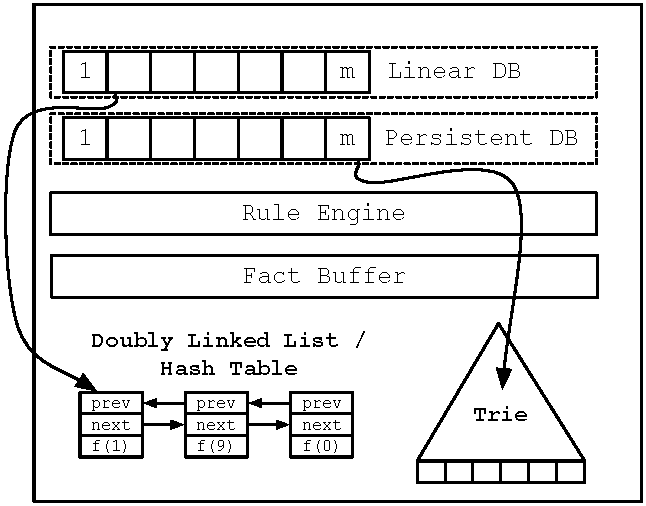
\includegraphics[width=0.5\textwidth]{figures/overview.pdf}
\end{center}
\caption{Layout of the node data structure. The critical part are the
   database structures: linear facts are storing using either doubly-linked lists or hash
tables while persistent facts are stored using tries.}
\label{fig:node}
\end{wrapfigure}

Fig.~\ref{fig:node} presents the overview of the node.  Each node of the graph
stores 4 main data structures: (1) the \emph{rule matching engine}, (2) a
\emph{fact buffer} for
storing incoming and temporary facts.  (3) the \emph{database of linear facts}, and (4)
the \emph{database of persistent facts}.

The rule engine maintains a simplified view of the two databases and efficiently
decides which rules need to be executed. For instance, if a rule $r_1$ needs
facts \texttt{a} and \texttt{b} to be applied and the database already contains
\texttt{a} facts, once a \texttt{b} fact is derived by another rule, the rule
engine is informed and then schedules $r_1$ to be executed. Our compiler is
responsible for the code that is executed when a rule is scheduled.  A compiled
rule contains instructions to search and match facts from the database and then
derive new facts if the body of the rule is successfully matched.

\subsection{Database Data Structures}\label{sec:data_structures}

The organization of the data structure is critical because logical facts can be
retracted and asserted frequently. This means that the database needs to allow
fast insertions and deletions but also needs to have reasonably fast mechanisms
for lookup. The database of facts is partitioned by predicate, therefore, each
predicate can have its own data structure depending on the patterns of access
for that particular predicate. Linear predicates are stored using the
following data structures:

\begin{itemize}
   \item \emph{Doubly-Linked List Data Structures}. Each linear fact is a node
   of the linked list. Allows constant
   $\mathcal{O}(1)$ insertion and deletion of facts given the pointer of the
   target node. Although lookup operations take linear time, this is not a huge
   disavantage since most predicates tend to have a small number of facts.
   \item \emph{Hash Table Data Structures}. For predicates with many facts that
   require expensive and repetitive lookup operations using a specific argument
   (i.e., searching for facts with a concrete value), linked lists are too slow.
   Hash tables build upon lists by hashing facts using a specific argument and
   then using separate chaining with doubly-linked lists for collision
   resolution. Hash tables are, on average, $\mathcal{O}(1)$ for insertion,
   deletion and lookup, however they require more memory.
\end{itemize}

For persistent tuples, we use \emph{Trie Data Structures}, which are trees where
facts are indexed by a common prefix. Since persistent facts are never deleted,
it's not expensive to index facts by a common prefix, which also tends to save
memory in the long run.
